\documentclass[12pt]{article}
\usepackage{setspace}
\usepackage{amsmath}
\usepackage{graphicx}
\usepackage[margin=1.0in]{geometry}
\usepackage[usenames,dvipsnames]{color}
\usepackage{hyperref}

\renewcommand{\familydefault}{\sfdefault}

\title{Proposed formula for COMP airdrop to early users}
\author{Produced by @allthecolors in collaboration with the Compound user community}

\begin{document}

\maketitle

\section{Introduction}

This document describes a proposed formula for determining the amount of COMP
to distribute to addresses that interacted directly with the Compound protocol
prior to the release of the COMP token and distribution model.

For further context about the rationale and degree of support for this idea
in the community, please see the
\href{https://www.comp.xyz/t/should-compound-retroactively-airdrop-tokens-to-early-users/595}{Relevant discussion on the Compound Forums}.


\section{Formula Details}

The two strategies for allocating an airdrop to early users that have clear traction
in the forums are:
\begin{itemize}
  \item{\textbf{socially-weighted}: every qualifying address receives a fixed amount of COMP}
  \item{\textbf{capital-weighted}: COMP received per address depends on the value of
        assets supplied and borrowed to the protocol, possibly relative to the total
        value locked (TVL) in the protocol, over time}
\end{itemize}
There are valid arguments in favor of both approaches. The UNI airdrop featured
a combination of the two: socially-weighted for all interacting non-contract addresses
(even including would-be users whose transactions failed!),
plus a capital-weighted distribution to liquidity providers.
\\\\
The proposed formula is therefore a simple linear combination of
socially-weighted and capital-weighted terms, with COMP awarded to user $i$ having the form

\begin{equation*}
\mathrm{COMP}_i = w\cdot\mathrm{socialCOMP}_i + \left(1-w\right)\cdot\mathrm{capitalCOMP}_i
\end{equation*}

The parameter $w$, $0 \leq w \leq 1$ controls what fraction of the distribution is allocated socially
and what fraction is allocated by capital, with $w=0$ being fully capital-weighted and $w=1$ being
fully socially-weighted. 

\subsection{Definition of a qualifying address}
\label{qualify}
Addresses qualifying for an early user airdrop under this proposal meet the following criteria:
\begin{itemize}
  \item{Issued at least one supply (\texttt{mint()}) or borrow (\texttt{borrow()}) transaction
        with Compound V1 money market contract or Compound V2 contracts in the following window:
        \begin{itemize}
           \item{First eligible block: Compound V1 launch on Sept 26, 2018 UTC (block \texttt{6400278})}
           \item{Last eligible block: one week prior to COMP token launch, June 8, 2020 UTC (block \texttt{10228172})}
        \end{itemize}
       }
  \item{Is an external owned account (EOA). This requirement includes all addresses that
        interacted directly with the protocol but excludes interactions that were mediated
        by contracts. A rationale for this criterion can be found in the forums (entry 214).}
  \item{Does not show evidence of participation in the Sybil attack on early governance; see
        \texttt{SybilAttackRemover.py} for address detection details.}
\end{itemize}

\subsection{Evaluation of social term} 

The social term simply takes the total COMP to be distributed and apportions it
equally to every qualifying address:

\begin{equation*}
  \mathrm{socialCOMP}_i = \frac{\mathrm{TotalCOMP}}{\textrm{Number of qualifying addresses}}
\end{equation*}

\subsection{Evaluation of capital term}

The Compound protocol would not have been able to scale to its current size without
the capital of its earliest users. The capital term is intended to recognize the
importance of early capital to the protocol by distributing COMP to addresses in
proportion to how much capital they supplied to (and possibly borrowed from) the
protocol over the early-user eligibility window.
\\\\
Compound currently uses an established capital-weighted formula for distributing
COMP to current suppliers and borrowers in the protocol. Here, a simpler model is
proposed in which the value supplied/borrowed by an address at each interaction
with the protocol is multiplied a simple TVL multiplier $m$ based on
when the interaction took place. This multiplier ranges linearly from $m = 1$
for interactions occurring at the end of the eligibility window to $m = 86$ at the
beginning of the eligibility window, where $m = 86$ represents the approximately 86-fold
increase in TVL for the Compound protocol during the eligiblity window.
\\\\
For each user $i$ and supply/borrow transaction $\alpha$, we estimate the capital
associated with the transaction $C_{i\alpha}$ by multiplying the amount of tokens
of type T, $N_{i\alpha,T}$ by the average price per token, $P_T$, over the eligibility window,

\begin{equation*}
  C_{i\alpha} = N_{i\alpha,T}P_T
\end{equation*}

where the average price per token for non-stablecoins is obtained from a simple two-point average
of the price at the beginning and end of the eligibility window according to CoinGecko,

\begin{equation*}
  \bar{P_T} = \frac{1}{2}\left[P_T(\textrm{Compound V1 launch date}) + P_T(\textrm{COMP token launch date})\right]
\end{equation*}

Average price per token for stablecoins is fixed at 1. 
A more accurate accounting could be achieved using daily price history data from Coingecko,
but we argue that the price histories of all tokens compatible with the protocol were
sufficiently nonvolatile during the eligibility window that this approximation does not
materially affect the calculation.
\\\\
For each transaction's capital value $C_{i\alpha}$, we account for its ``earliness'' by
computing the TVL multiplier $m_{i\alpha}$ described above from the block number $b_{\alpha}$ of the transaction,
\begin{equation*}
  m_{i\alpha} = 1 + k\frac{b_{\alpha} - b_{\textrm{end}}}
                     {b_{\textrm{start}}-b_{\textrm{end}}}
\end{equation*}
where $b_{\textrm{start}}$ and $b_{\textrm{end}}$ are the beginning and ending blocks of the
eligibility window, described in section \ref{qualify}, and $k=85$ is chosen so that each TVL
multiplier $m_{i\alpha}$ satisfies $1 \leq m_{i\alpha} \leq 86$ as described above.
\\\\
With this information, the capital term for address $i$ is computed by taking the product
of the capital value $C_{i\alpha}$ and the TVL multiplier $m_{i\alpha}$ for each qualifying
transaction, summing over all transactions by that address, and dividing by the sum over all
qualifying addresses. The result is the fraction of $\textrm{TotalCOMP}$ 
apportioned to address $i$, so we multiply by $\textrm{TotalCOMP}$ to convert from a unitless
fraction to a total denominated in COMP.
\begin{equation*}
  \mathrm{capitalCOMP}_i = \textrm{TotalCOMP}\cdot\left[\frac{\sum\limits_{\textrm{transactions }\alpha}{m_{i\alpha}C_{i\alpha}}}{\sum\limits_{\textrm{users }j}\left({\sum\limits_{\textrm{transactions }\alpha}{m_{j\alpha}C_{j\alpha}}}\right)}\right]
\end{equation*}

\subsection{``Top-up'' adjustment to \textrm{TotalCOMP}}

Any nonzero value of the weight factor $w$ will produce a COMP distribution with a ``floor'',
that is, a minimum number of COMP that every qualifying address will receive.
To help align the distribution with the governance goals of the airdrop,
we propose to include a ``top up'' quantity of COMP, distributed equally to all qualifying
addresses, to raise this floor to an integer number. By setting the floor at an integer 
number, any future proposals to support early user participation in governance
(e.g. decreasing the minimum COMP required to submit a CAP) will be easier for the
community to understand and implement. This ``top-up'' adjustment effectively
increases the amount of COMP to be distributed by some small inflationary factor,
which this proposal aims to keep modest (below 10\%).

\subsection{Selection of the social-vs-capital weight parameter $w$}

Given community support for both capital-based and social-based weights,
$w$ should be neither 0 nor 1, but something in between. A natural starting
point for conversation is $w = 0.5$, which places equal weight on the two terms.
\\\\
A 50-50 weight scheme has the apparent advantage of splitting the difference
between these two philosophical approaches to early user rewards, but it has
several disadvantages that stem from the exponential features of capital:
\begin{itemize}
  \item{It distributes most of the early user rewards to deep-pocketed
        users whose "capital at risk" in the protocol may have been a
        relatively small {\em fraction} of their available capital,
        compared to smaller users who may have risked a considerably larger
        {\em fraction} of their available capital. It's unlikely that
        awarding the deepest-pocketed users most of the distribution will
        achieve the goal of increasing widespread early user participation
        in governance or overall project growth.}
  \item{It leaves the vast majority of early users with an amount of COMP
        insufficient to enable or motivate genuine participation in governance}
\end{itemize}

Community members interested in exploring how the choice of $w$ affects the
early user distribution list can run the script \texttt{EarlyUserProposal.weighted.py}
with different values of $w$ (expressed as an integer percentage between 0 and 100)
as the single argument and compare the outputs.
\\\\
The distribution that appears to best meet the goal of empowering the
early user community with a meaningful shot at a role in governance is
95\% socially-weighted, 5\% capital-weighted:

\begin{figure*}[h]
 \centering
 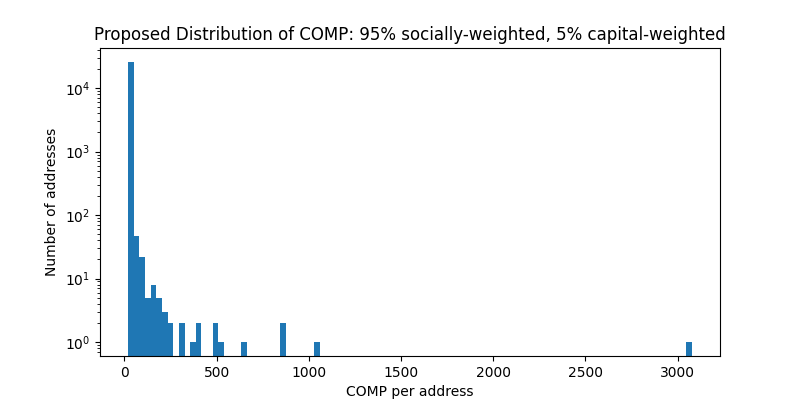
\includegraphics[width=5in]{proposals/Proposal.png}
\end{figure*}

Merits of this choice of $w$ include:
\begin{itemize}
  \item{The largest amount distributed to any single address ($\approx$ 3000 COMP) is roughly two orders of magnitude greater than the floor amount (20 COMP).}
  \item{More than 9 in 10 early users receive between 20 and 21 COMP, with fewer than 50 addresses receiving in excess of 100 COMP and only 2 addresses exceeding 1000 COMP.}
\end{itemize}

\section{References}
\begin{enumerate}
  \item{``Should Compound Retroactively Airdrop Tokens to Early Users?'' \href{https://www.comp.xyz/t/should-compound-retroactively-airdrop-tokens-to-early-users/595}{Compound Forum}.}
  \item{\texttt{CompEarlyUserAnalysis} \href{https://github.com/0xA1176ec01045/CompEarlyUserAnalysis}{repository on GitHub}, where the implementation and results are hosted.}
  \item{\href{https://raw.githubusercontent.com/0xA1176ec01045/CompEarlyUserAnalysis/main/proposals/Proposal.95-5.csv}{Proposed early user distribution of COMP by address}.}
\end{enumerate}
\end{document}
